\documentclass[oneside,a4paper,11pt]{report}
%\usepackage[T1]{slovak}
\usepackage[utf8]{inputenc}
\usepackage{latexsym}
\usepackage{graphicx}
\usepackage{amsmath}
\usepackage{caption}
\usepackage{fancyhdr}
%\usepackage{picins}
\usepackage{times}
\usepackage{mathptmx}
\usepackage{url}
\usepackage{booktabs}
\usepackage{appendix}

\pagestyle{fancy}
\fancyhead{}
\fancyhead[C]{\leftmark}
\renewcommand{\chaptermark}[1]{\markboth{\thechapter.\ #1}{}}


\usepackage[Sonny]{fncychap}
\makeatletter
 \ChNameVar{\small}
 \ChNumVar{\LARGE}
 \ChTitleVar{\LARGE\centering}
 \ChRuleWidth{0.05pt}
 \ChNameUpperCase

%\title{Štúdium premenných hviezd vo vysokoenergetickej části spektra}
\title{Study of variable stars in high energies }

\author{Matúš Kocka}



\begin{document}
%\begin{figure}
%\begin{center}
%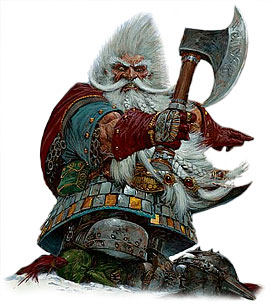
\includegraphics[width=6cm]{the-white-dwarf}
%\end{center}
%\end{figure}
%\pagebreak
\tableofcontents

\addcontentsline{toc}{chapter}{\protect\numberline{}Introduction}
\chapter*{Introduction}

.... pindy o CVs a SNe 

\chapter{Cataclysmic variable stars }

 
\section{Magnetic cataclysmic variable stars }
\subsection{Polars}
\subsection{Intermediate polars}
\subsection{Galactic population ofcataclysmic variables }
\label{GXRE}

\chapter{Model of post shock region}
\section{Thermal bremstalung}




\section{PSR}
%\section{Hmotnosť bieleho trpaslík}
%\subsection{Pomocou kontinua}
%\subsection{Pomocou K železných čiar}
%\chapter{Spracovanie dát}
%\section{INTEGRAL}
%\section{XMM-Newton}
%\chapter{Určenie hmotností vybraných IP}



%\chapter{Intermedialne polary}   




\begin{thebibliography}{99}
\addcontentsline{toc}{chapter}{\hspace*{6mm}Literatúra}
\bibitem {(Warner 1995)} Warner, B. 1995, Cataclysmic Variables, (Cambridge: Cambridge Univ. Press)


\end{thebibliography}


\appendix
\section*{Appendix}
this will be the appendix
%\pagebreak
%\thispagestyle{empty}
%\LaTeX{}
\end{document}
